\section{Trajectory Planner}\label{CHAP: Method}

\begin{itemize}
    \item Tidligere kjent som 'Method'.
    \item Har lyst å skrive litt om tankegangen bak utviklingen, ikke bare om hvordan ting endte opp med å bli.
    \item Ingen 'Preliminaries', alt av forkunnskaper og antagelser burde vært gjort rede for i 'Background'.
    \item Spesifikt mitt arbeid.
    \item Tar det fra start til slutt. 
    \subitem Persistent variables \& settings.
    \subitem COLREGs assessment.
    \subitem Dynamic Horizon.
    \subitem Casadi setup (generer F)
    \subitem Feasibility check.
    \subitem Initial conditions and Reference LOS guidance.
    \subitem NLP init.
    \subitem Main loop, med alt som skjer der.
    \subitem Solve NLP, give output.
    \item Bit for bit, forklar hva, hvorfor, hvordan, eventuellt andre versjoner eller ideer som ble prøvd.
    \item forklar informasjonsflyt, kanskje som eget delkapittel. 
    \item My method is NOT a dock-to-dock system, the developed algorithm is NOT suitable for stationkeeping or docking maneuvers.
    Dock-To-Dock does exist see \cite{WärtsiläDockToDock}, 
    otherwise there are OTHER algorithms more suitable for docking. (TODO: FIND SOMETHING TO CITE)
\end{itemize} 



\iffalse
The developed algorithm is a path following trajectory planner and collision avoidance package where the dynamics of the \gls{OS}
vessel are formulated as an ODE (TODO: REF TIL EQ) and the optimal trajectory is found by a method called direct multiple shooting.
CasADi is employed to 

The developed algorithm is a path following trajectory planner and collision avoidance package where the dynamics of the \gls{OS} vessel
are modelled as ODEs and used together with a designed cost function to formulate an \gls{OCP}. The \gls{OCP} is solved numerically
by transforming the problem into a \gls{NLP} with the help of a CasADi framework and a method called direct multiple shooting, 

numerically
through a direct multiple shooting method via a CasADi framework using an \gls{IPOPT} solver.
\fi

(TODO: skriv bedre og mer korrekt.)
This chapter presents the development of the trajectory planning and collision avoidance algorithm, explaining the design decisions made
and analyzing some of the problems that arose during development. First the general dataflow of the algorithm is explained so that
an intuition is formed as for how the individual parts are connected. Second a piece by piece construction of the algorithm up until
the construction of the \gls{NLP}. Lastly the \gls{NLP} is constructed and solved using framework provided by CasADi. The core design
of the algorithm is that path following is done through numerical optimization of a cost function, whilst collision avoidance and safety
is implemented as hard constraints in the \gls{NLP}, together an optimal trajectory is formed. 


\subsection{Dataflow}
\iffalse
\begin{itemize}
    \item Begin by explaining the idea behind how the algorithm should work.
    \item This chapter will need diagrams.
    \subitem input $\rightarrow$ ??? $\rightarrow$ output
    \subitem show how the internal functions parse data
    \item Serves as a good overview of the whole algorithm.
\end{itemize}
\fi
The dataflow is depicted in Figure \ref{FIG: Dataflow chart}, to avoid clutter the diagram does not include every subfunction and minor detail, it's a
representative diagram, not a blueprint. On the left we begin with a higher level system, the algorithm
relies on getting information about it's own vessel, as well as information about other ships (called Tracks in the diagram), static obstacles and miscellaneous
other settings. These structs need to contain data in some specific fashions which will be discussed more deeply later in this chapter.(TODO: This part).
The Tracks structure as it arrives from the higher lever system is assumed to have full prediction, the algorithm can simplify the prediction
for testing purposes but there is no internal logic to switch between prediction detail level. Regardless of if the tracks were simplified or not
they are parsed through a \gls{COLREGs} assessment algorithm  to determine which \gls{Ts}s need to be considered active obstacles, as well as
finding how long until the \gls{tCPA}, and which \gls{COLREGs} situation the encounters would be.
Independently of the creation of dynamic obstacles we use the information about our own vessel's position and end goal
to determine how long the time horizon for this instance of the algorithm should be. When time horizon and discretization step size
is known the CasADi setup can be ran to generate the function 'F' which will be used during the construction of the \gls{NLP} later.
With a dynamic horizon in place a LOS algorithm can be used to generate the final piece of the dynamic obstacles struct; the trajectory of the \gls{Ts}s
themselves, which are used to place constraints later in the \gls{NLP} construction. One crucial detail to take note of is that COLREGs assessment of a \gls{Ts}
is conducted using only the waypoints provided by the Tracks struct, while the placement of dynamic constraints are based on the trajectory generated by a LOS
guidance law. 
\iffalse
possible encounters with a dynamic obstacle
is predicted using only a handful of set waypoints from the tracks struct, while the placement of the dynamic constraints are based on the a LOS guidance law
trajectory.
\fi
The feasibility check is not ran in the first instance of the algorithm after starting up the system. The result of the feasibility check
is used when generating our \gls{OS}'s reference path to determine if the desired velocity should be reduced. the LOS guidance
returns as mentioned the positions for the dynamic obstacles constraints as well as the reference positions and velocities in NED.

The \gls{NLP} can now be initialized. Initial position and velocity forms the first constraint of the \gls{NLP} (TODO: SKRIV MER)




\begin{figure}
    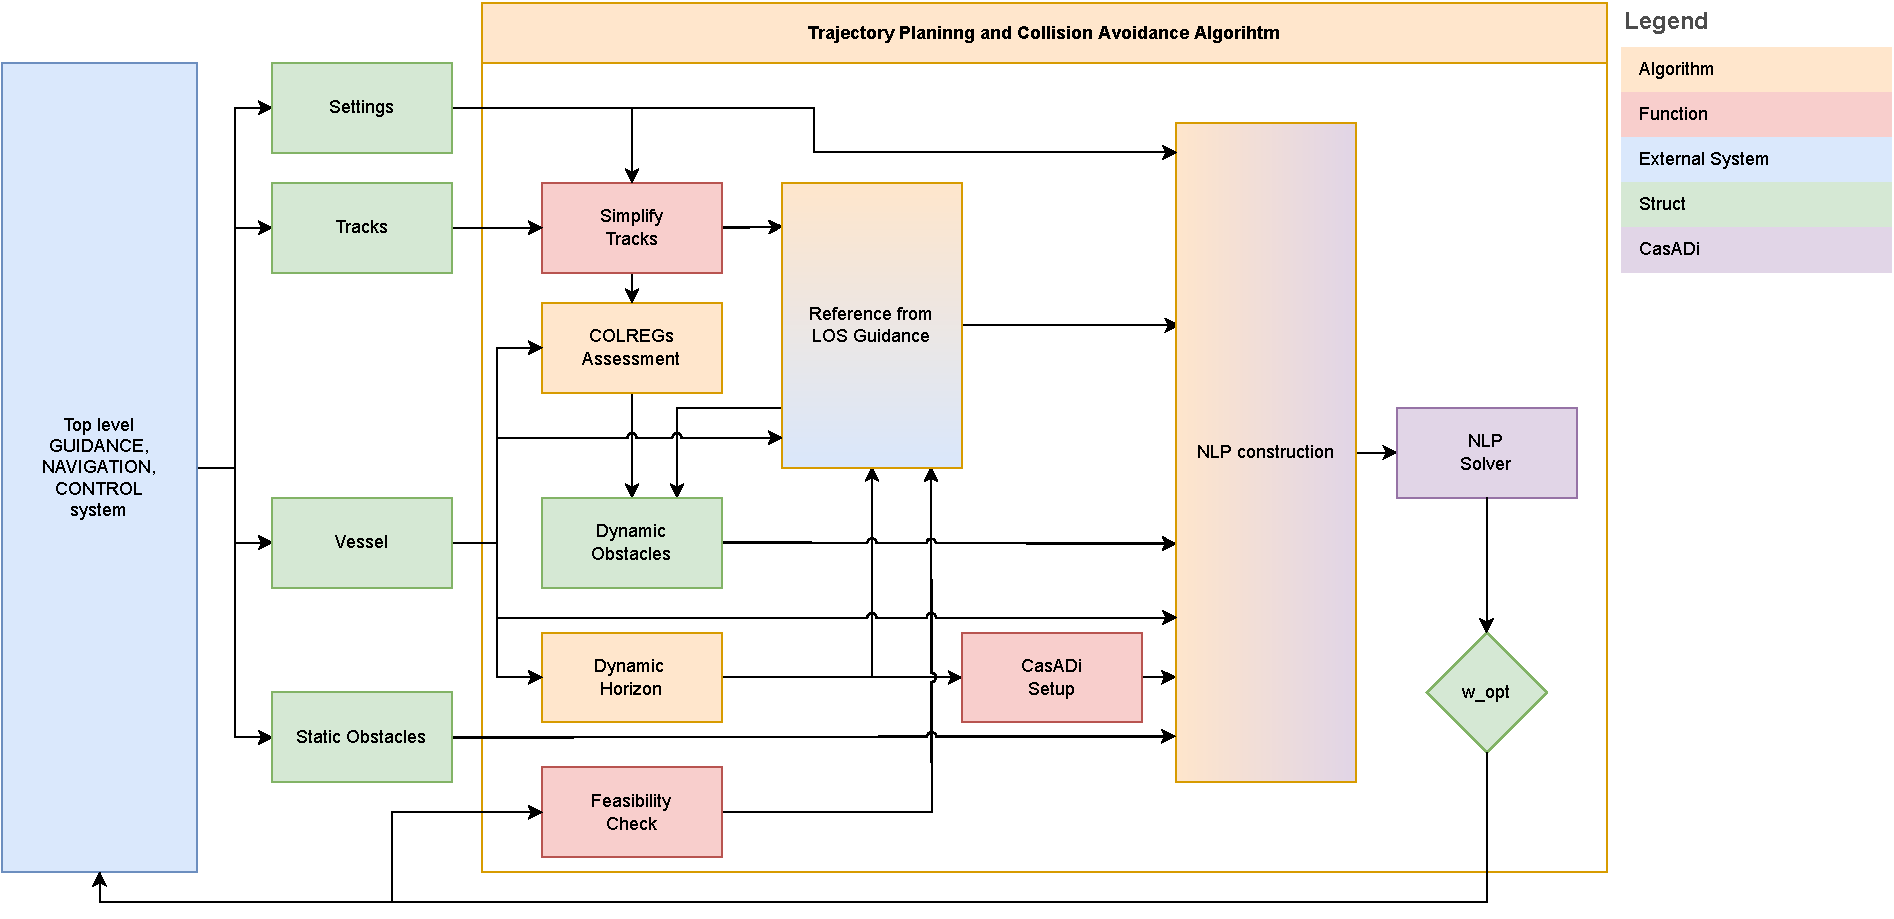
\includegraphics[width=\textwidth]{Images/SimpleSystem.pdf}
    \caption{(TODO: skriv)The simple version of the dataflow...}
    \label{FIG: Dataflow chart}
\end{figure}

\subsection{Setup}
\begin{itemize}
    \item All the stuff before main loop.
    \item subsubsection for each 'block' as outlined by the dataflow.
\end{itemize}

\begin{itemize}
    \item when the trajectory planner is called we need to run through some calculations before constructing the NLP problem
    \item These calcualtions are a mix of situation analysis, simulation settings, and CasADi initialization.
    \item Some of these calculations could be redundant in a complete control and navigation system,
    where other modules of the system would calculate the same thing.
    \item It's also important to remember that the value of many parameters are just guesswork, many of the subfunctions
    would benefit from a more sophesticated design that are tuned based on the situation the vessel finds itself in.
\end{itemize}

\subsubsection{Simplify Prediction}
%Avansert TS prediction må skrives om i background.
%Tracks struct må forklares i background.
This part of the setup is only required in simulations, the aim is to emulate the 'standard' way target ship (TS) prediction is conducted,
which is to say constant course and velocity [TODO: Citation needed]. The TS trajectory is changed so that the first waypoint is the current position of the
ship, and the next waypoint is one nautical mile in the direction of the ships heading. Ideally course over ground would be used instead of heading, however
in the simulator crab angle and sideslip are not accounted for, therefor heading and course are the same angle.
Excess waypoints stored in the TS struct are also truncated and the current waypoint index is forcefully set to 1 to prevent index out of range type errors.


\subsubsection{COLREGs assessment}
The COLREGs assessment function solves two problems; figuring out if\/when a TS vessel will be in close enough proximity that evasive maneuvers might be considered,
and deciding which of the COLREGs rules will apply for the encounter. The design idea is to first find what the distance at closest point (dCPA) of approach with the TS is, and then
time until cloest point of approach (tCPA) occurs. If both dCPA and tCPA values are under a set threshold we consider the encounter an active event and run the
COLREGs situation assessment shown by \cite{Thyri2021b}. %COLREGs assessment is also explained in [TODO: fordypningsoppgaven].

Finding the dCPA and tCPA between two vessels with constant velocity and course is easily done with a formula as shown by(eller in?) \cite{Kufoalor2018}.
%%%%%(TODO: SKRIV OM ALT DETTE, TING BLE FLYTTET HERFRA TIL KAPITTEL 2.3) %%%%%



%However with our wish for more advanced target ship prediction this formula is not sufficient on it's own.
%In order to achieve 'full coverage' of our intended path,
%nd the projected path of the target ship, we must check the dCPA and tCPA starting at each waypoint in the path of both vessels.
% helper function 'getCPAlist' is constructed to get the list of all dCPAs and their respective tCPAs when given two agent structs (AGENT STRUCTS MÅ FORKLARES I BACKGROUND) as inputs.
%o achieve full coverage the getCPAlist function is ran twice so that the perspective of each agent is considered. 

%In terms of code the function for COLREGs assessment uses the helper function getTCPAlist, which in turns uses three more helper functions. The first helper function vesselReadout
%returns the position and velocity in NED given a vessel struct and waypoint index as input. whereisTS gives the same output but takes an agent and time as input arguments instead.
%Lastly the function ClosestApproach takes the output from vesselReadout and whereisTS and applies the equations \eqref{eq:tCPAdCPA}. The dCPA, tCPA and positions are stored and the
%waypoint index is incremented by one, repeat until all waypoints 

TODO: Ikke ferdig


to get a list of all dCPA and tCPAs between two agents, as well as the corresponding positions of both
agents as they are when the euqations \eqref{eq:tCPAdCPA} are used. getCPAlist 

\begin{algorithm}[t]
    \caption{getCPAlist. Denne ble jævelig stygg, beholder den for synlighet}\label{alg:getCPAlist}
    \begin{algorithmic}[1]
    \Require{$Agent1. Agent2$}\Comment{Agent is a struct that includes path waypoints}
    \State $dCPAlist \gets []$
    \State $tCPAlist \gets []$
    \State $pos\_OS\_list \gets []$
    \State $pos\_TS\_list \gets []$
    \State $timer \gets 0$ \Comment{Initialize timer used to calculate position of Agent2}
    \For{$i \gets Agent1.current\_wp : agent\_wplist\_length - 1$}
        \State $[pos_{OS}, vel_{OS}] \gets VesselReadout(Agent1, i)$ \Comment{VesselReadout explained in algorithm...}
        \State $DisttonextWP \gets $Distance to Agent1's next waypoint
        \State $TimetonextWP \gets DisttonextWP \div$ Agent1's speed over ground
        \State $[pos_{TS}, vel_{TS}] \gets whereisTS(Agent2, Timer)$ \Comment{whereisTS explained in algorithm...}
        \State $[dCPA, tCPA] \gets$ Equation for dCPA \& tCPA as shown by...
        \State $tCPA \gets tCPA + timer$ \Comment{Add travel time to reach current wp}
        \State $timer \gets timer + TimetonextWP$
        \State $pos\_OS\_list \gets [pos\_OS\_list, pos_{OS}]$ \Comment{Append all values to respective list.}
        \State $pos\_TS\_list \gets [pos\_TS\_list, pos_{TS}]$
        \State $dCPAlist \gets [dCPAlist, dCPA]$ 
        \State $tCPAlist \gets [tCPAlist, tCPA]$ 
        \State $i \gets i + 1$
    \EndFor
    \State \textbf{return} $pos\_OS\_list, pos\_TS\_list, dCPAlist, tCPAlist$
    \end{algorithmic}
\end{algorithm}

\subsubsection{Dynamic Horizon}
\begin{itemize}
    \item Dynamic horizon is a balancing act between distance to goal, encompassing all active dynamic obstacles, and not looking to far ahead into the future.
    \item changing the dynamic horizon is really just changing how many control intervals we want the NLP to have.
    \item As the distance to goal approaches zero we want the number of control intervals to shrink accordingly, otherwise we end up with too many control intervals stationary at the goal, which can cause problems like the cost function becoming unbalanced.
    \item If there are active dynamic obstacles we need the dynamic horizon to encompass them.
    \item we don't want the dynamic horizon to be too short during transit (why not?).
\end{itemize}

\subsubsection{CasADi setup}
\begin{itemize}
    \item sym x = [N, E, psi, u, v, r]
    \item sym tau as a free variable
    \item sym xref as reference
    \item model parameters
    \item M, C, D matrix
    \item xdot \= [nu\_dot, eta\_dot]
    \item Error in the correct reference frame.
    \item Why is the cost function the way it is.
    \item runge-kutta method.
    \item the final function F that CasADi needs.
    \item Noe av disse greiene blir dekt av Background, forhåpentligvis.
\end{itemize}

\subsubsection{Feasibility check}
\begin{itemize}
    \item The feasibility check came from the wish to read out the status report CasADi prints to the command window.
    \item It's very important to know if the previous iteration of the trajectory planner function yielded a feasible result or not.
    \item if the result is not feasible the path forward might be completely blocked, in which case reducing our vessel speed is the best option.
    \item Very simple check, just checks if every point in the previously calculated optimal trajectory is within 5 meters of each other. This is very lenient and should of course change depending on vessel speed.
\end{itemize}

\subsubsection{Reference from LOS}
\begin{itemize}
    \item I didn't write this \:)
    \item The important part is that the time discretization is consistent with the trajectory planner's time step
    \item You don't need to use LOS for reference.
    \item Position reference and speed reference need to be consitent with each other.
\end{itemize} 


\subsection{NLP Construction and Solver}
\begin{itemize}
    \item inputs\: vessel, ref\_trajectory, static\_obs, dynamic\_obs, F, settings, h, N, previous\_w\_opt.
    \item sub funksjoner\:
    \subitem Dynamic Obs.
    \subitem Static Obs.
    \subitem integration step.
    \item output\: w\_opt
\end{itemize}

\subsubsection{NLP initialization}
\begin{itemize}
    \item Initial conditions and end of interval coditions, we need the end of one control interval and the beginning of the next to match.
    \item Tror dette delkapittelet er litt unødvendig
\end{itemize}

\subsubsection{Integration step}
\begin{itemize}
    \item Getting the correct reference
    \item make sure all the indexes are correct!
    \item put the references in w0, speeds up runtime significantly.
\end{itemize}

\subsubsection{Dynamic Obstacles constraints}
\begin{itemize}
    \item When to place constraints
    \item Where to place them
    \item How to place them
\end{itemize}

\subsubsection{Static Obstacles constraints}
\begin{itemize}
    \item Explain static\_obstacles\_check and the theory for convex-free set
    \item explain why circles, such as the ones used for dynamic obstacles are insufficient.
    \item this is sort of similar to finding a cross track error, if that helps to explain what is going on.
\end{itemize}

\begin{figure}
    \centering
    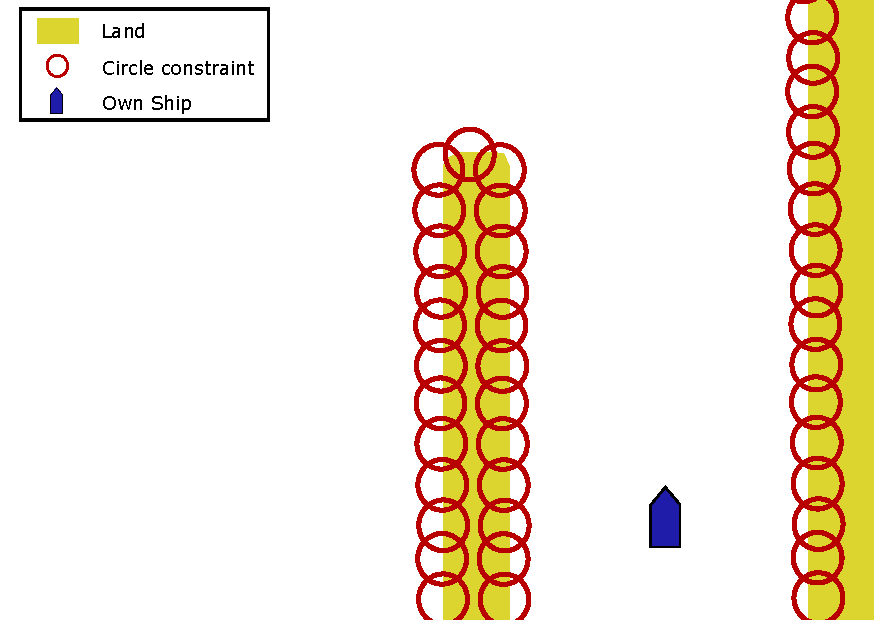
\includegraphics[width=\textwidth]{Images/StaticObs_Naive.pdf}
    \caption{TODO: SKRIV OG REFERER. Naiv approach 1}     \label{FIG: Static Obs Naive approach 1}
\end{figure}

\begin{figure}
    \centering 

    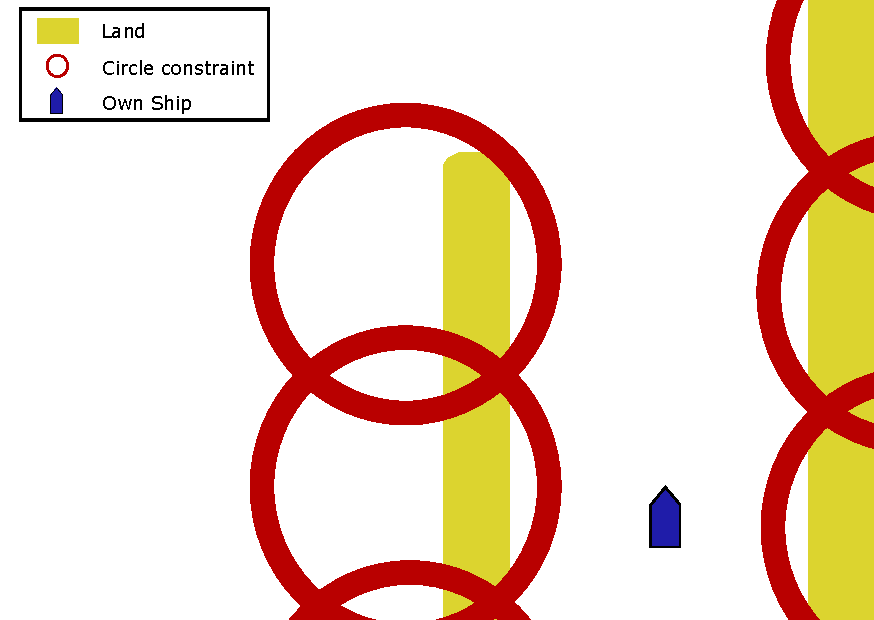
\includegraphics[width=\textwidth]{Images/StaticObs_Naive2.pdf}
    \caption{TODO: SKRIV OG REFERER. Naiv approach 2}     \label{FIG: Static Obs Naive approach 2}
\end{figure}

\begin{figure}
    \centering
    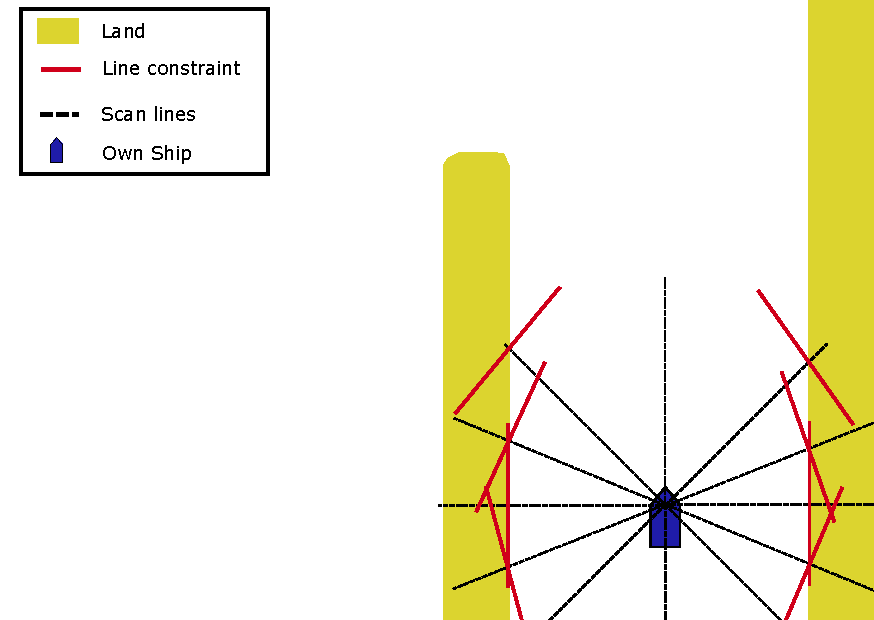
\includegraphics[width=\textwidth]{Images/StaticObs_lines.pdf}
    \caption{TODO: SKRIV OG REFERER. Convex free set}     \label{FIG: Static Obs Lines}
\end{figure} 

\subsubsection{Solver}
\begin{itemize}
    \item Options, there are many options.
    \item things to try / were tried for optimizing runtime.
    \item CasADi really does all the hard work.
\end{itemize}

\subsection{Alternative Ideas and Lessons}
Burde kanskje heller gå under discussion, og igjen i future work.
\begin{itemize}
    \item Change w0 based on previous solution runtime.
    \item Gamle versioner av Static\_obs.
    \item eksperimenter med feasibility check.
    \item Masse styr med COLREGs assessment, tcpa og dcpa.
    \item ipopt innstillinger.
\end{itemize}
\newpage